\begin{exr}
$f$ est une fonction définie sur $\R$ dont le tableau de variations est :

	\begin{tikzpicture}
	\tkzTabInit{$x$/0.5,$f(x)$/1.25}{$-\infty$,$-1$,$2$,$+\infty$}
	\tkzTabVar{+/$2$,-D-/$-\infty$/$-\infty$,+/$-1$,-/$-\infty$}
	\end{tikzpicture}
	
	Donner les limites indiquées dans le tableau et les équations des  asymptotes à $\Crbf$ que l'on peut en déduire.
 \end{exr}
%
%
%
\begin{exr}On considère une fonction $f$. Compléter les phrases :
	\begin{enumerate}
	\item Si $\limite{x\to +\infty}{f(x)}=-\infty$ alors tout intervalle  \dots
	\item Si $\limite{x\to -\infty}{f(x)}=3$ alors tout intervalle  \dots
	\item Si $\limite{x\to +\infty}{f(x)}=+\infty$ alors tout intervalle  \dots
	\item Si $\limite{\substack{x\to 10 \\ x<10 }}{f(x)}=-\infty$ alors tout intervalle  \dots
	\end{enumerate}
\end{exr}
%
%
%
\begin{exr}
Soit $f$ la fonction définie sur $\R$ par $f(x)=\frac{6}{\Exp^x+3}$.

Déterminer les asymptotes de $\Crbf$ par le calcul.
\end{exr}
%
%
%
\begin{exr}
Déterminer les limites suivantes :
	\begin{enumerate}
	\item 
		\begin{enumerate-}[label=\alph*.](2)
		\item $\limite{x\to+\infty}{(5x^2-3)(4-3\sqrt{x})}$
		\item $\limite{x\to-\infty}{x^{15}+x^{6}-10}$
		\item $\limite{x\to+\infty}{x^3-5x^2+4x\sqrt{x}-6}$
		\item $\limite{x\to-\infty}{x^3-5x^2+3x+4}$
		\end{enumerate-}
	\item 
		\begin{enumerate-}[label=\alph*.](2)
		\item $\limite{x\to-\infty}{\frac{3x^2-5x+7}{4x^3-6x-7}}$
		\item $\limite{x\to+\infty}{\frac{3x^3-5x+7}{4x^2-6x-7}}$
		\item $\limite{x\to-\infty}{\frac{5x^3+4x-3}{2x^3+3}}$
		\item $\limite{x\to+\infty}{\frac{2x+3\sqrt{x}}{3x-2\sqrt{x}}}$
		\end{enumerate-}
	\item 
		\begin{enumerate-}[label=\alph*.](3)
		\item $\limite{\substack{x\to2\\x<2}}{\frac{10-7x}{4x-2}}$
		\item $\limite{\substack{x\to-1\\x>-1}}{\frac{x+3}{-x^2+x+2}}$
		\item $\limite{\substack{x\to0\\x<0}}{\frac{\Exp^x+3}{\Exp^x-1}}$
		\end{enumerate-}
	\item 
		\begin{enumerate-}[label=\alph*.](3)
		\item $\limite{x\to+\infty}{(4x-5)\Exp^x}$
		\item $\limite{x\to-\infty}{\mleft(4-\frac3x\mright)\mleft(2\Exp^x-5\mright)}$
		\item $\limite{x\to+\infty}{\mleft(\frac4{x^2}-5\mright)\mleft(1-3\Exp^x\mright)}$.
		\item $\limite{x\to-\infty}{\mleft(3x^2-4+5\Exp^x\mright)}$
		\item $\limite{x\to+\infty}{\mleft(3x^2-5x+\Exp^x\mright)}$
		\item $\limite{x\to-\infty}{\frac{2\Exp^x-3}{4-5\Exp^x}}$
		\item $\limite{x\to+\infty}{\frac{2\Exp^x-3}{4-5\Exp^x}}$ 
		\end{enumerate-}
	\end{enumerate}
\end{exr}


\begin{exr}
Voici la courbe représentative d'une fonction $f$ définie sur $\R\setminus\{-2;1\}$ :
\begin{centered}
\begin{tikzpicture}[x=0.5cm,y=0.5cm]
\drawrepere{-7,5,-6,8}
\draw[line width=2pt] plot[samples=1000,domain=-7:-2.01] function {(2*(x+0.5)**2-0.25*(x-0.5))/((x+2)*(x-1))};
\draw[line width=2pt] plot[samples=1000,domain=-1.99:0.99] function {(2*(x+0.5)**2-0.25*(x-0.5))/((x+2)*(x-1))};
\draw[line width=2pt] plot[samples=1000,domain=1.01:5] function {(2*(x+0.5)**2-0.25*(x-0.5))/((x+2)*(x-1))};
\node[above] at (2,-4){$\Crbf$};
\end{tikzpicture}
\end{centered}
Déterminer graphiquement les limites de $f$ en $-\infty$, en $+\infty$, en $-2$ et en $1$ à gauche et à droite.

Indiquer les asymptotes éventuelles.
\end{exr}
%
%
%
%
%
%
\begin{exr}
On considere la fonction définie sur $\R$ par $f(x)=\dfrac{ax^2+bx+c}{x^2+1}$ où $a$, $b$ et $c$ sont trois réels.\\
La courbe $\Crbf$ est donnée ci-dessous.
\begin{centered}
\begin{tikzpicture}[x=0.5cm,y=0.75cm]
\drawrepere{-8,10,-1,6}
\draw[line width=2pt] plot[samples=1000,domain=-8:10] function {(5*x**2+x+2)/(x**2+1)};
\node[above] at (3,5){$\Crbf$};
\end{tikzpicture}
\end{centered}
	\begin{enumerate}
	\item 
		\begin{enumerate}
		\item Calculer les limites en $-\infty$ et $+\infty$ de $f(x)$.
		\item En déduire, à partir du graphique, la valeur de $a$.
		\end{enumerate}
	\item Déterminer, à partir du graphique, les valeurs de  $c$ puis $b$.
	\end{enumerate}
\end{exr}
%
%
%
\begin{exr}
Voici la courbe représentative d'une fonction $f$ définie sur $\R$ :
\begin{centered}
\begin{tikzpicture}[x=0.75cm,y=0.5cm]
\drawrepere[add to x clip end=2.5pt,add to y clip end=2.5pt]{-4,8,-3,5}
\draw[line width=2pt,-{Circle[length=5pt]},shorten >=-2.5pt] plot[samples=1000,domain=-8:6] function {0.05*x**3+0.01*x**2-1.08*x-0.05};
\node[below] at (4,-1){$\Crbf$};
\draw[line width=2pt,{Circle[length=5pt,open,line width=1pt]}-,shorten <=-2.5pt] (6,2)--(8,3);
\end{tikzpicture}
\end{centered}

Cette fonction est-elle continue ?
\end{exr}
%
%
%
\begin{exr}
Voici la courbe représentative d'une fonction $f$ définie sur $\R$ :
\begin{centered}
\begin{tikzpicture}[x=1cm,y=0.4cm]
\drawrepere[add to x clip end=2.5pt,add to y clip end=2.5pt]{-4,5,-5,5}
\draw[line width=2pt] plot[samples=1000,domain=-3.5:4.2] function {0.33*x**3-0.38*x**2-3.44*x + 1.67};
\node[above] at (2,-4){$\Crbf$};
\end{tikzpicture}
\end{centered}

Cette fonction est-elle continue ?
\end{exr}

%
%
%
\begin{exr}
Voici la courbe représentative d'une fonction $f$ définie sur $\R^*$ :
\begin{centered}
\begin{tikzpicture}[x=1cm,y=0.4cm]
\drawrepere{-5,5,-5,5}
\draw[line width=2pt] plot[samples=1000,domain=-5:-0.1] function {x+1/x};
\draw[line width=2pt] plot[samples=1000,domain=0.1:5] function {x+1/x};
\node[above] at (2,-4){$\Crbf$};
\end{tikzpicture}
\end{centered}

Cette fonction est-elle continue sur $\R$ ? sur $\R-*$ ? sur $\R*$ ?
%non continue sur $\R$ car une fonction ne peut être continue que là où elle est définie et $f$ n'est pas définie en $0$.
\end{exr}

\begin{exr}
Calculer les limites suivantes.
	\begin{enumerate}
	\item $\lim\limits_{x\to-\infty}\frac{4x^3-3x+2}{3x^4+1}$
	\item $\lim\limits_{x \to +\infty}\frac{x^2+x-3}{x+2}$
	\item $\lim\limits_{\substack{x\to -2\\x<-2}}\frac{x^2+x-3}{x+2}$
	\item $\lim\limits_{\substack{x\to 3\\x>3}}\frac{x+1}{x^2-4x+3}$
	\end{enumerate}
\end{exr}

\begin{exr}
On considère une fonction $f$ définie sur $\R+*$ telle que : $-\frac1x+1\leqslant f(x)\leqslant \frac1x+1$ pour tout réel $x>0$.
	\begin{enumerate}
	\item Déterminer, si possible, la limite de $f$ en $+\infty$.
	\item Déterminer, si possible, la limite de $f$ en $0$.
	\end{enumerate}
\end{exr}

\begin{exr}
Soit $f$ la fonction définie sur $\R\setminus\{1\}$ par $f(x)=\frac{2x+\cos x}{x-1}$. On note $\Crbf$ sa courbe dans un repère orthonormé.
\begin{enumerate}
\item \'Etudier la limite de $f$ lorsque $x$ tend vers $1$.
\item
    \begin{enumerate}
    \item Démontrer que : $\frac{2x-1}{x-1}\leqslant f(x)\leqslant \frac{2x+1}{x-1}$ pour tout réel $x>1$.
    \item En déduire la limite de $f$ quand $c$ tend vers $+\infty$.
    \item Donner la limite de $f$ quand $x$ tend vers $+\infty$ sans jusitifications.
    \end{enumerate}
\item Interpréter graphiquement les résultats obtenus aux questions précédentes.
\item \'Etudier la position relative de $\Crbf$ par rapport à la droite d'équation $y=3$.
\end{enumerate}
\end{exr}

\begin{exr}
Étudier les limites suivantes :

\begin{enumerate-}(4)
\item $\lim\limits_{x\rightarrow +\infty}\left(x+\dfrac{1}{x}\right)$.
\item $\lim\limits_{x\rightarrow -\infty}x^2(x-6)$
\item $\lim\limits_{x\rightarrow +\infty}\left(x^2+1\right)(2-x)$
\item $\lim\limits_{x\rightarrow +\infty}\sqrt{x}(1-x)$
\item $\lim\limits_{x\rightarrow +\infty}\left(2\mathrm{e}^{x}-1\right)$
\item $\lim\limits_{x\rightarrow -\infty}\left(\dfrac{1}{x-5}\right)$
\item $\lim\limits_{x\rightarrow -\infty}\left(\dfrac{1}{x^2+1}+7\right)$
\item $\lim\limits_{x\rightarrow -\infty}\left(\dfrac{2}{x}-3\right)$
\end{enumerate-}
\end{exr}

\begin{exr}
Étudier les limites suivantes :

\begin{enumerate-}(3)
\item $\lim\limits_{x\rightarrow 0}\dfrac{x}{\sqrt{x}-3}$
\item $\lim\limits_{\substack{x\rightarrow 5\\x>5}}\dfrac{1}{x-5}$
\item $\lim\limits_{\substack{x\rightarrow 3\\x>3 }}\dfrac{x+1}{x-3}$
\end{enumerate-}
\end{exr}

\begin{exr}
Calculer :

\begin{enumerate-}(3)
\item $\lim\limits_{x\rightarrow -\infty}\left(3x^2-4x+7\right)$
\item $\lim\limits_{x\rightarrow +\infty}\left(3x^2-4x+7\right)$
\item $\lim\limits_{x\rightarrow +\infty}\left(2x^4-7x+8\right)$
\item $\lim\limits_{x\rightarrow +\infty}\left(\dfrac{3x+5}{7x-2}\right)$
\item $\lim\limits_{x\rightarrow -\infty}\left(\dfrac{x^2+2}{1-x}\right)$
\end{enumerate-}
\end{exr}

\begin{exr}
Soit $g$ la fonction définie sur $\R$ par $g(x)=\frac{2-x^2}{x^2+1}$.

La courbe représentative $\Crbf{g}$ de $g$ admet-elle une asymptote ? Si oui, laquelle ?
\end{exr}

\begin{exr}
Déterminer les limites en $-\infty$ et $+\infty$ des fonctions définies par les expressions suivantes :

\begin{enumerate-}[label=\alph*.](2)
\item $f(x)=\dfrac{x^2+2}{1-x}$
\item $g(x)=\dfrac{x+3}{-2x^2+1}$
\end{enumerate-}
\end{exr}

\begin{exr}Déterminer les limites suivantes :

\begin{enumerate-}[label=\alph*.](3)
\item $\lim\limits_{\substack{x\rightarrow 2\\x>2}}\dfrac{x}{3x-6}$
\item $\lim\limits_{\substack{x\rightarrow 2\\x<2}}\dfrac{x}{3x-6}$
\item $\lim\limits_{\substack{x\rightarrow 4\\x>4}}\dfrac{x^2}{4-x}$
\item $\lim\limits_{\substack{x\rightarrow 4\\x<4}}\dfrac{x^2}{4-x}$
\item $\lim\limits_{\substack{x\rightarrow 0\\x<0}}\left(4+\dfrac{1}{x}-\dfrac{2}{x^2}\right)$
\item $\lim\limits_{\substack{x\rightarrow 0\\x>0}}\left(4+\dfrac{1}{x}-\dfrac{2}{x^2}\right)$
\end{enumerate-}
\end{exr}

\begin{exr}
Voici la courbe représentative d'une fonction.
\begin{centered}
\begin{tikzpicture}[x=0.5cm,y=0.5cm]
\drawrepere{-7,9,-5,5}
\draw[line width=2pt] plot[samples=200,domain=-10:-2.02] function {(x+1)/((x+2)*(x-3))};
\draw[line width=2pt] plot[samples=200,domain=-1.992:2.99] function {(x+1)/((x+2)*(x-3))};
\draw[line width=2pt] plot[samples=200,domain=3.01:10] function {(x+1)/((x+2)*(x-3))};
\node[left] at (2,1){$\Crbf$};
\end{tikzpicture}
\end{centered}
Conjecturer les limites suivantes :
	\begin{enumerate-}[label=\alph*.](3)
	\item $\lim\limits_{x\rightarrow -\infty}f(x)$
	\item $\lim\limits_{x\rightarrow +\infty}f(x)$
	\item $\lim\limits_{\substack{x\rightarrow -2\\x<-2}}f(x)$
	\item $\lim\limits_{\substack{x\rightarrow -2\\x>-2}}f(x)$
	\item $\lim\limits_{\substack{x\rightarrow 3\\x<3}}f(x)$
	\item $\lim\limits_{\substack{x\rightarrow 3\\x>3}}f(x)$
	\end{enumerate-}
\end{exr}


\begin{exr}
On considère la fonction définie sur $ \R$ par 
$f(x)=\begin{cases}2x-1\text{ si }x\leqslant 1\\x^2\text{ si }>1\end{cases}$.
	\begin{enumerate}
	\item Représenter graphiquement cette fonction.
	\item $f$ est-elle continue sur $ \R$ ? Justifier par un calcul.
	\end{enumerate}
\end{exr}
%
%
%
\begin{exr}
On considère la fonction définie sur $ \R$ par 
$f(x)=\begin{cases}\mathrm{e}^{x}\text{ si }x\leqslant 0\\x+2\text{ si }>0\end{cases}$.
	\begin{enumerate}
	\item Représenter graphiquement cette fonction.
	\item $f$ est-elle continue sur $ \R$ ? Justifier par un calcul.
	\end{enumerate}
\end{exr}
%
%
%
\begin{exr}
On considère la fonction définie sur $ \R$ par 
$f(x)=\begin{cases}x^2-2x+3\text{ si }x\leqslant 3\\m\text{ si }>32\end{cases}$.
	\begin{enumerate}
	\item Pour quelle(s) valeur(s) de $m$ la fonction $f$ est-elle continue sur $ \R$ ?
	\item Représenter alors graphiquement  la courbe représentative de $f$ pour la ou les valeur(s) de $m$ trouvée(s) précédemment.
	\end{enumerate}
\end{exr}

\endinput
